\documentclass[10pt]{beamer}
\mode<beamer>{%
  \usetheme[]{CambridgeUS}}
\usepackage{geometry}
\usepackage{tikz}
\usepackage{amsfonts, amsmath, amssymb}
%\usepackage{dcolumn, multirow}
\usepackage{graphicx}
%\usepackage{anysize, indentfirst, setspace}
\usepackage{mathtools}
\usepackage{caption, rotating}
\usepackage{booktabs}
\usepackage{xcolor}
\usepackage{hyperref}
\usepackage{amsmath}
\usepackage{amssymb}
\usepackage{color}
\usepackage{mathabx}
\usepackage{sidecap}
%\usepackage{hanging}
%\usepackage{float}
\setlength{\tabcolsep}{3pt}

\title{Who Raises Environmental Justice in Rulemaking?\\Do Agencies respond?}
\author[Devin Judge-Lord]{Devin Judge-Lord}
\institute{University of Wisconsin}

%\titlegraphic{\includegraphics[width=20mm]{USTL}}
\date{\today}
\begin{document}


\begin{frame}<handout:0>
  \titlepage
\end{frame}

\section{Motivation}

\begin{frame}
\frametitle{1994}

``Addressing disproportionately high and adverse human health or environmental effects of programs, policies, and activities on minority populations and low-income populations.''

\bigskip
\centering

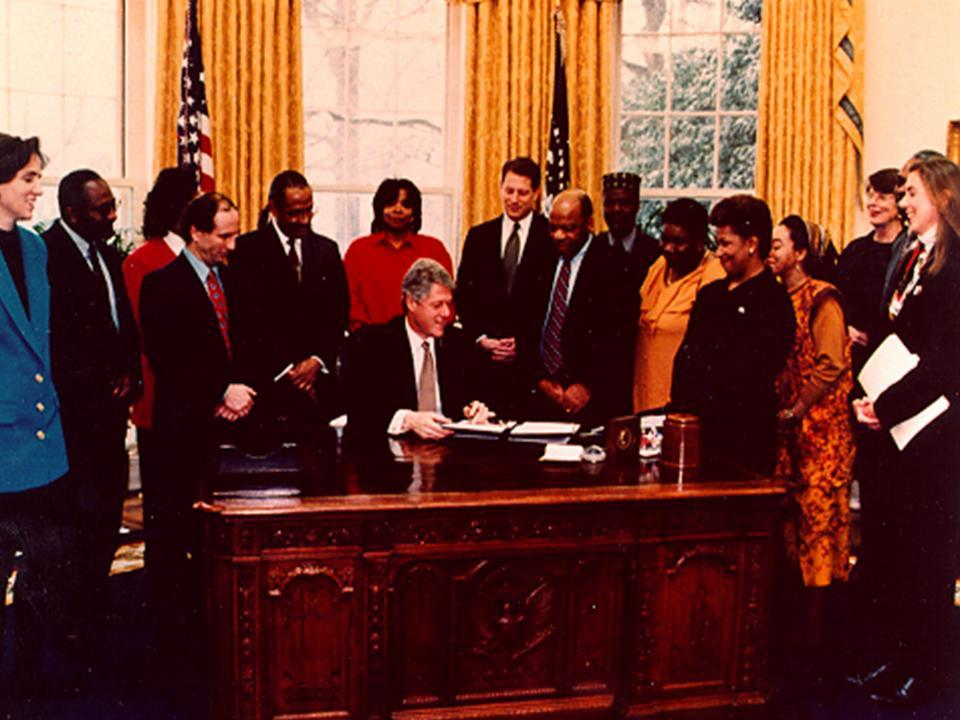
\includegraphics[width = 7cm]{clinton-ej.jpg}
\end{frame}


\begin{frame}
\frametitle{2002}
\centering
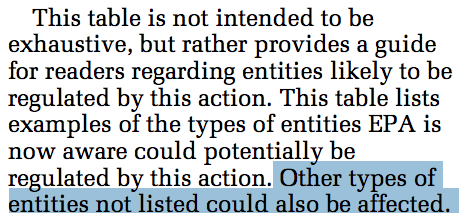
\includegraphics[]{ej_murcury_nprm.png}
\end{frame}

\begin{frame}
\frametitle{2002}

Comment: Heather McCausland, Alaska Community Action on Toxics (ACAT):

\bigskip

``The amount of methyl-mercury and other bio accumulative chemicals consumed by Alaskans (especially Alaskan Natives) could potentially be much higher than is assumed...The Alaska Native mortality rate for babies which according to the CDC is 70\% higher than the United States average. Indigenous Arctic \& Alaskan Native populations are some of the most polluted populations in the world (http://www.amap.no/). Global transport \& old military sites contaminate us too''
\end{frame}

\begin{frame}
\frametitle{2005}
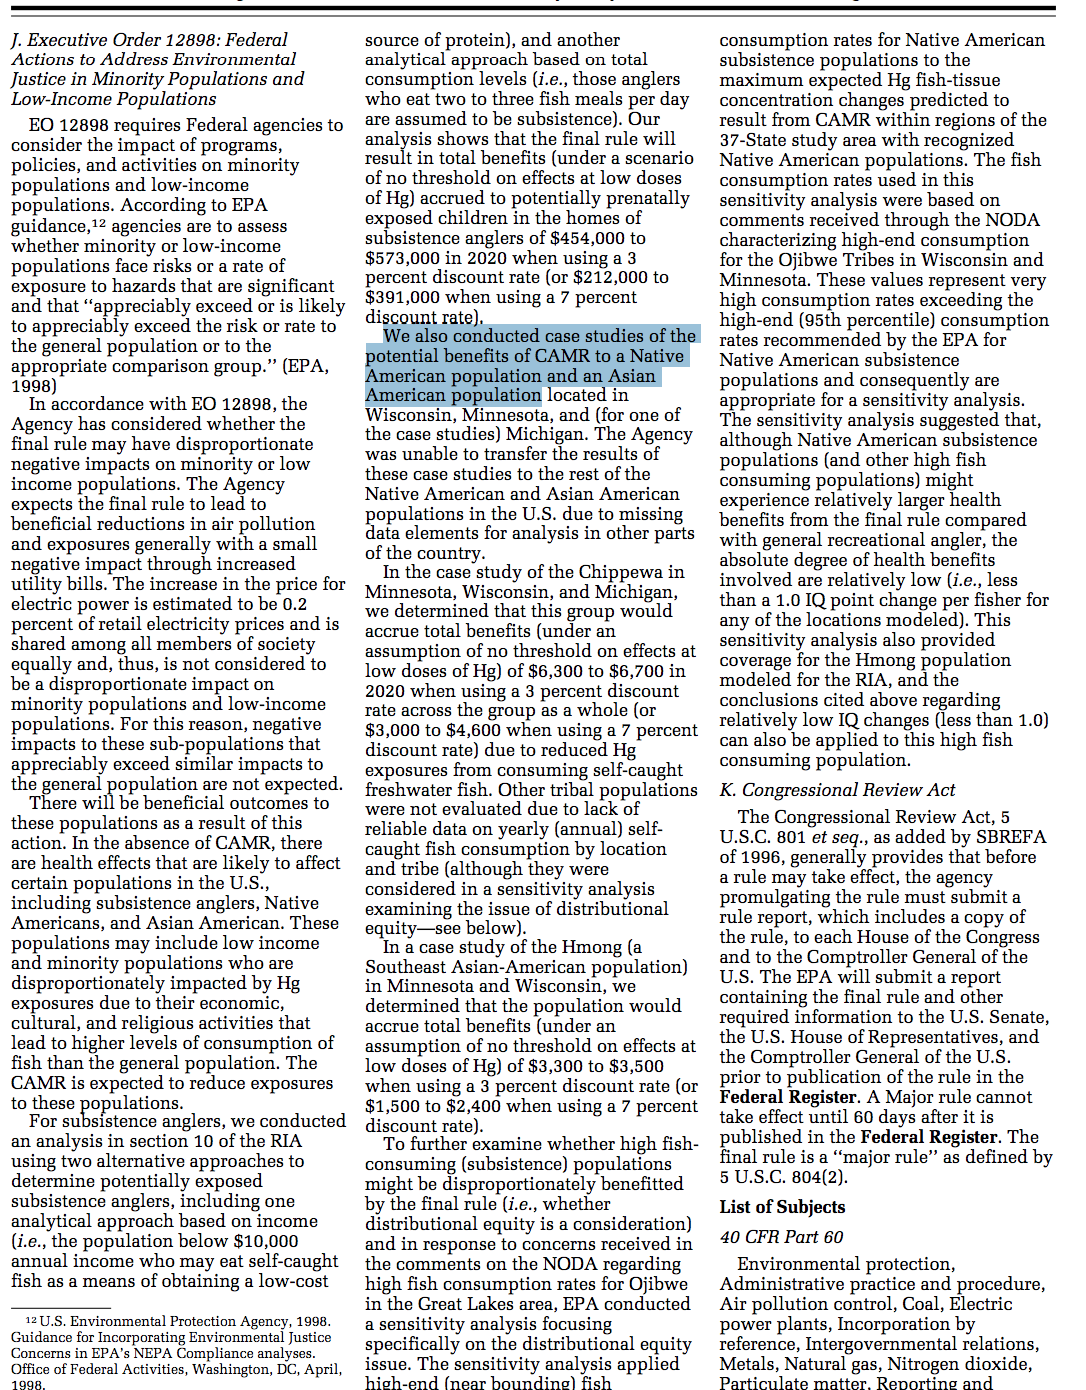
\includegraphics[width = \textwidth]{ej_murcury_final.png}
\end{frame}

\begin{frame}
\frametitle{2017}
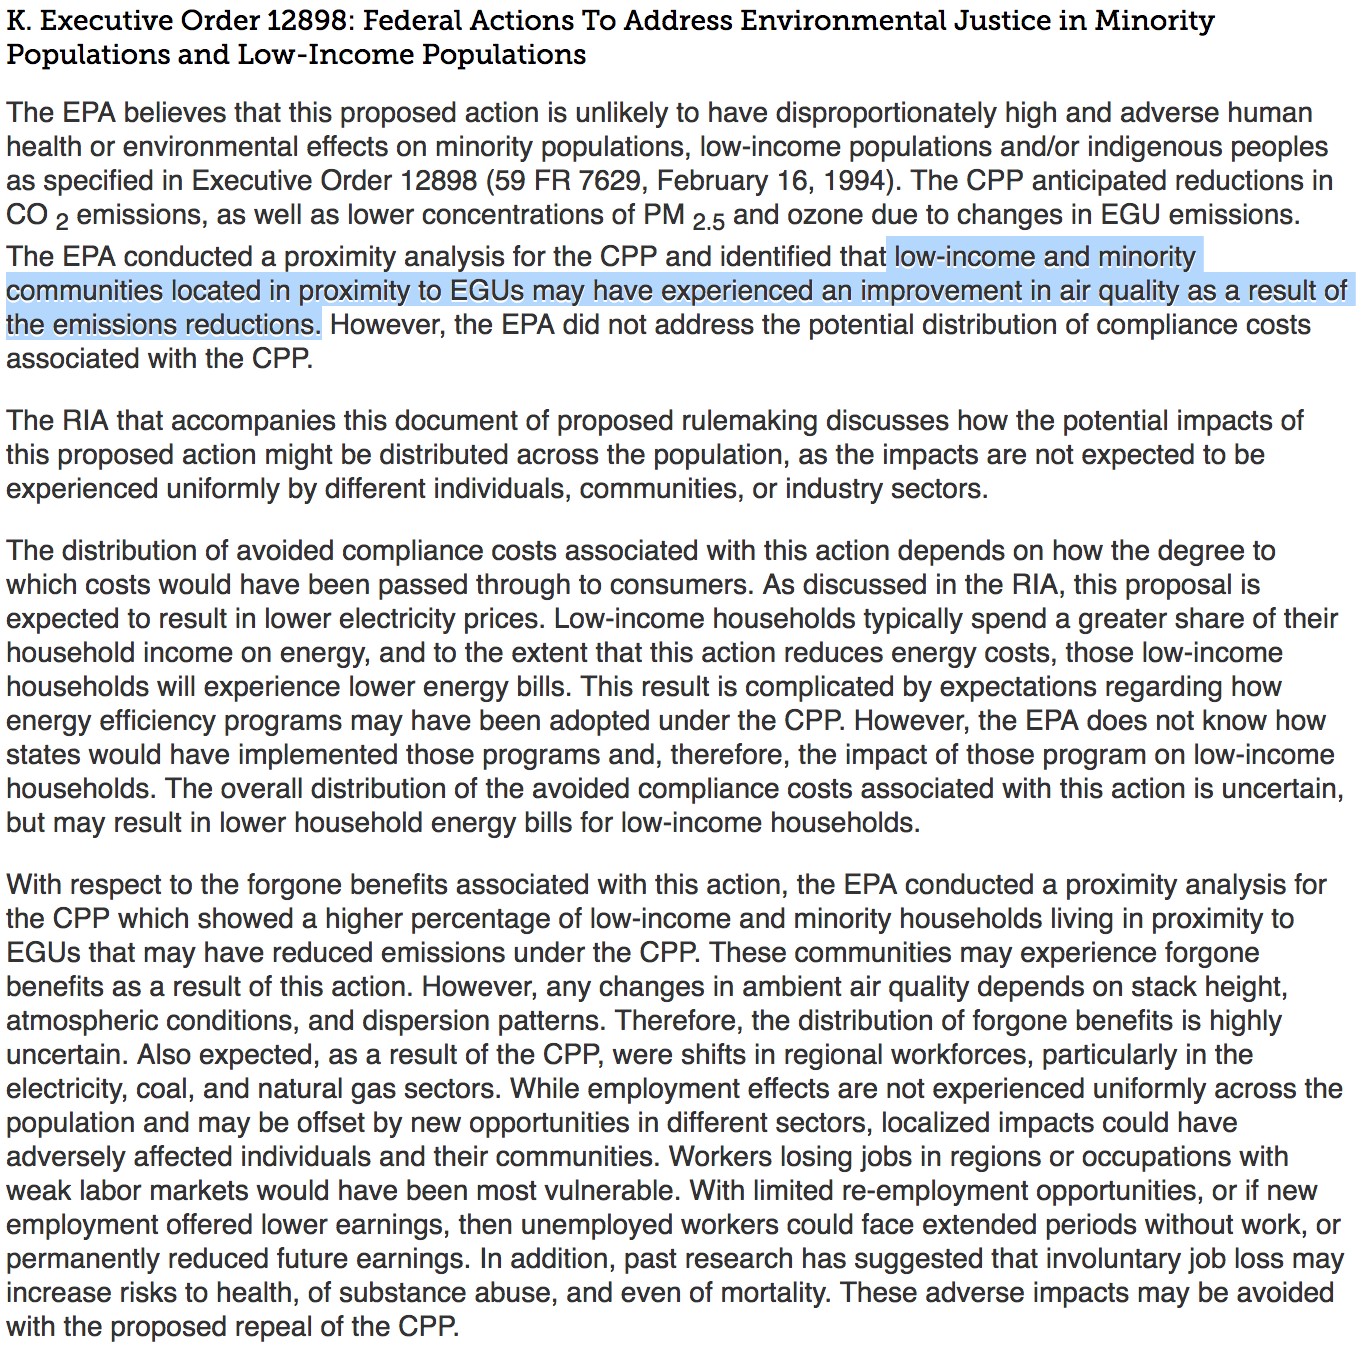
\includegraphics[width = \textwidth]{ej_murcury_repeal.png}
\end{frame}



\section{Theory}

\begin{frame}
\frametitle{Broader Argument}

Rulemaking constructs
\begin{itemize}
\item a political community of “relevant stakeholders” 
\item contested definitions of the public good and minority rights 
\item “appropriate” criteria to evaluate policy consequences
\end{itemize}


\end{frame}


\begin{frame}
\frametitle{Why would comments matter?}

Direct: information \& framing
\begin{itemize}
\item Facts (Wagner 1993) 
\item Minority opinion (Gillion 2013)
\item Appropriateness (March and Olson 2004)
\end{itemize}

Indirect: incentives \& threats
\begin{itemize}
\item Congressional or Presidential Attention (Yackee 2006, Yaver 2017)
\item Litigation (Coglanese 2001)
\end{itemize}
\end{frame}

\begin{frame}
\frametitle{Why do we care?}

Deserving groups

\bigskip

Criteria for allocating resources and protection

\bigskip

Voice vs. information 


\end{frame}

\begin{frame}
\frametitle{Why Focus on Environmental Justice?}

Increasing joint organizing (e.g. Checker 2005) 

\bigskip

Relatively unambiguous

\end{frame}


\section{Data}

\begin{frame}
\frametitle{Public Comments}
\begin{figure}
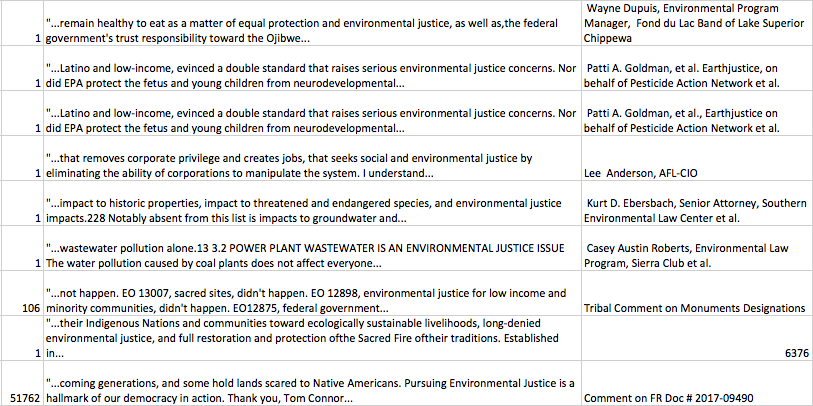
\includegraphics[width = \textwidth]{ejsample2}
\end{figure}
\end{frame}

\begin{frame}
\frametitle{Public Comments}
\begin{figure}
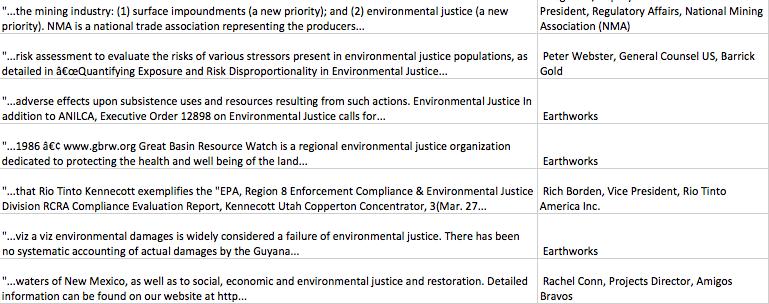
\includegraphics[width = \textwidth]{ejsample}
\end{figure}
\end{frame}


\begin{frame}
\frametitle{Public Comments}
\begin{figure}
\caption{Common Words in Online Comments (Left) and Attachments (Right}
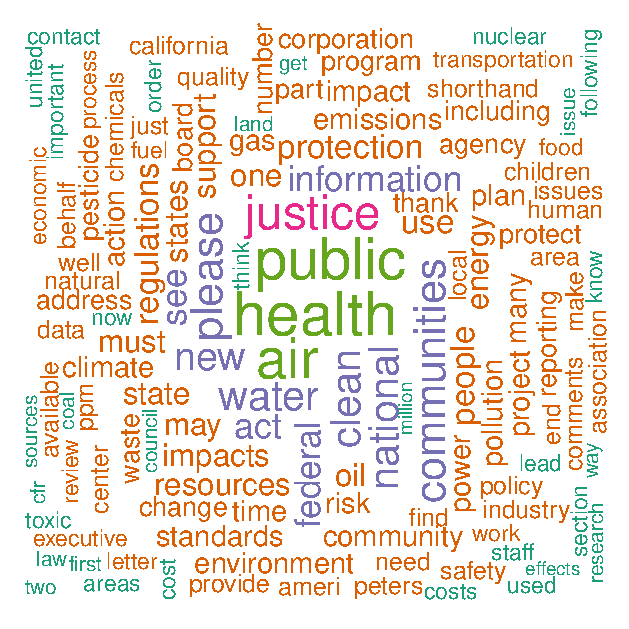
\includegraphics[width = \textwidth/2]{ej_wordcloud_comments.pdf}
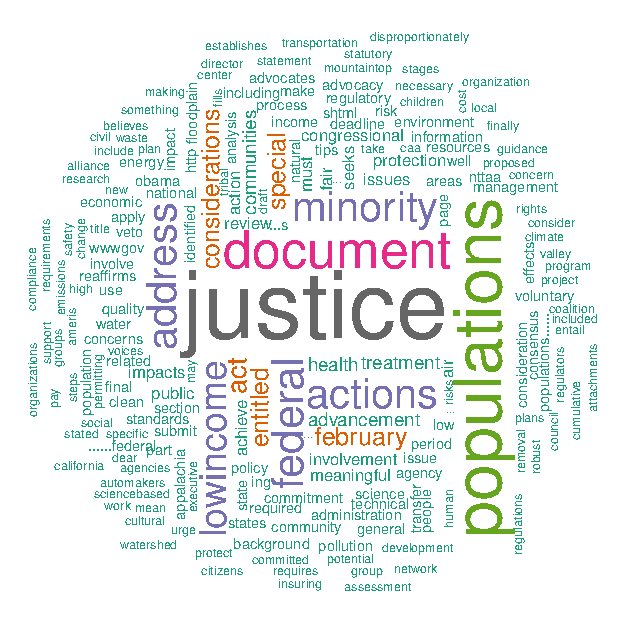
\includegraphics[width = \textwidth/2]{ej_wordcloud_attachments.pdf}
\end{figure}
\end{frame}


\section{Methods}

\begin{frame}
\frametitle{Procedure}
\begin{enumerate}
\item Retrieve all drafts, comments, and rules mentioning ``environmental justice''
\item Retrieve all draft and final rules from all agencies in above sample
\item Match rule drafts, comments, and final rules
\item Predict commenter race using census data
\item Logit Regression
\end{enumerate}
\begin{align*}
  \hat{EJ in Final} =
  \begin{array}{lll}
    1 & if &  \beta_0 + \beta_1 EJ in Draft + \beta_2 EJ in Comments + \\ & & \beta_3 Total Comments  + \epsilon > 0\\
0 & else &  
  \end{array}
\end{align*}

\end{frame}

\begin{frame}
\frametitle{Second-order Representation}
\begin{figure}[!h]
\centering
\begin{tabular}{rlll}
  \hline
 & Organization & Comments & Rules \\ 
  \hline
1 & Earthjustice & 1114782 & 28 \\ 
  2 & Natural Resources Defense Council &  340554 &  8 \\ 
  3 & Sierra Club &  349841 &  5 \\ 
  4 & Alliance for Climate Protection &  253867 &  5 \\ 
  5 & WE ACT for Environmental Justice &    2402 &  3 \\ 
  6 & CREDO &  112879 &  2 \\ 
  7 & Union of Concerned Scientists &   43559 &  2 \\ 
  8 & Earthworks &     308 &  2 \\ 
  9 & Communities for a Better Environment &      21 &  2 \\ 
  10 & Southern Company &       8 &  2 \\ 
  11 & Move On &  165948 &  1 \\ 
  12 & Care2 &   70450 &  1 \\ 
  13 & The Pew Charitable Trusts &   63769 &  1 \\ 
  14 & Hudson-Environmental Action &   35000 &  1 \\ 
  15 & Democracy for America &    4426 &  1 \\ 
  \end{tabular}
  \label{fig:orgs}
  \end{figure}

\end{frame}

\begin{frame}
\frametitle{Commenter Race}
\begin{figure}
\caption{Estimated Racial Distribution from Census Surnames}
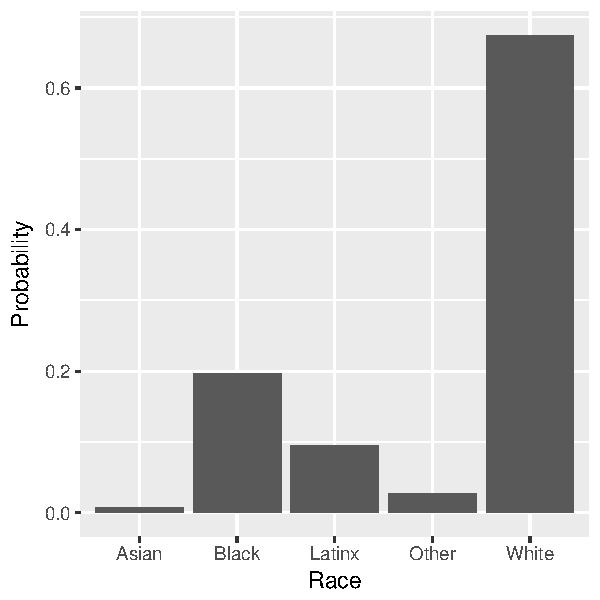
\includegraphics[width = \textwidth/2]{race_prob.pdf}
% 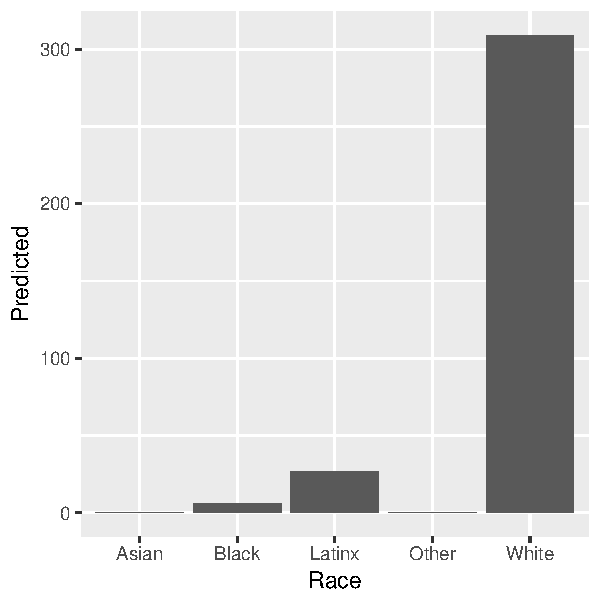
\includegraphics[width = \textwidth/2]{race_pred.pdf}
\end{figure}
\end{frame}


\begin{frame}
\frametitle{Commenter Race}
\begin{figure}
\caption{Common Words by Race}
\begin{tabular}{ccc}
White & Latinx & Black\\
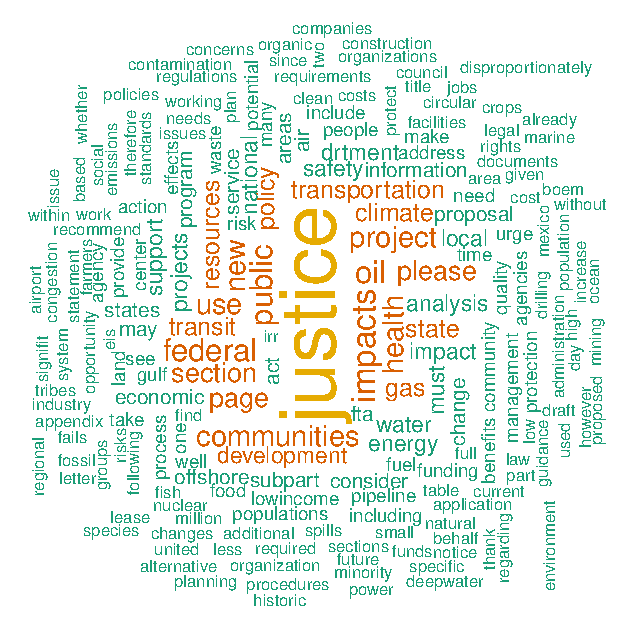
\includegraphics[width = \textwidth/3]{ej_white_words.pdf}
&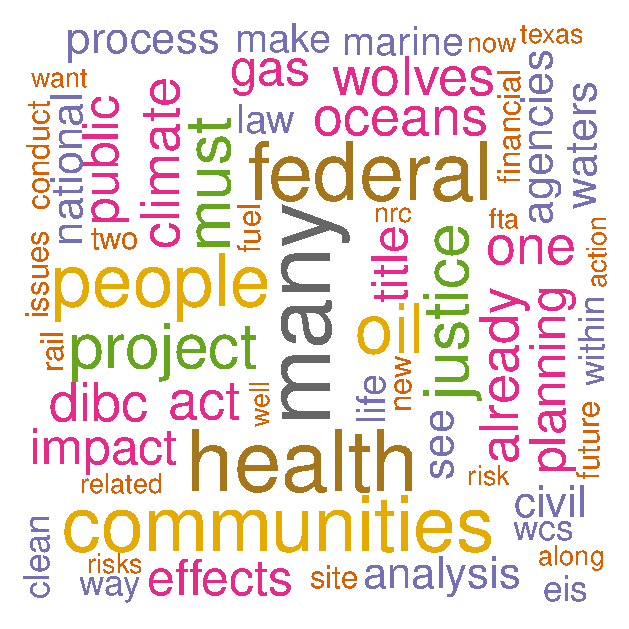
\includegraphics[width = \textwidth/3]{ej_latinx_words.pdf}
&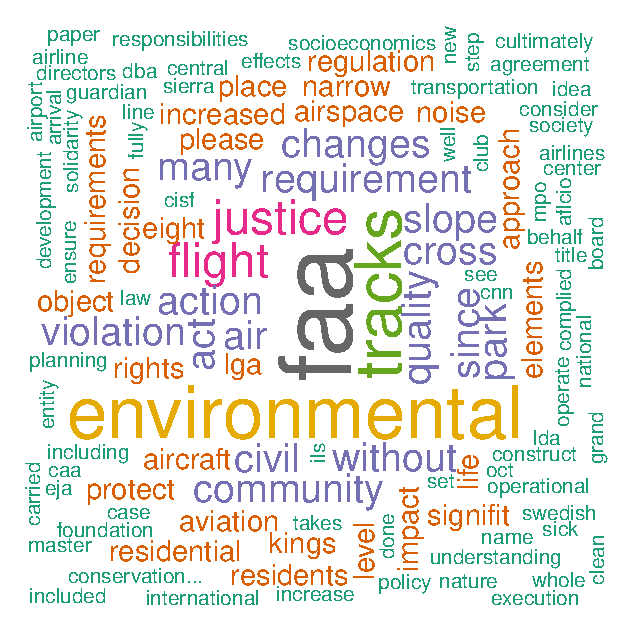
\includegraphics[width = \textwidth/3]{ej_black_words.pdf}
\end{tabular}
\end{figure}
\end{frame}


\begin{frame}
\frametitle{Public Comments}
\begin{figure}
\caption{Number of Rules where Environmental Justice Appears in the Record (Left) and Number of Comments per Notice or Proposed Rule (Right). Text indicates the agency for the most commented on rules.}
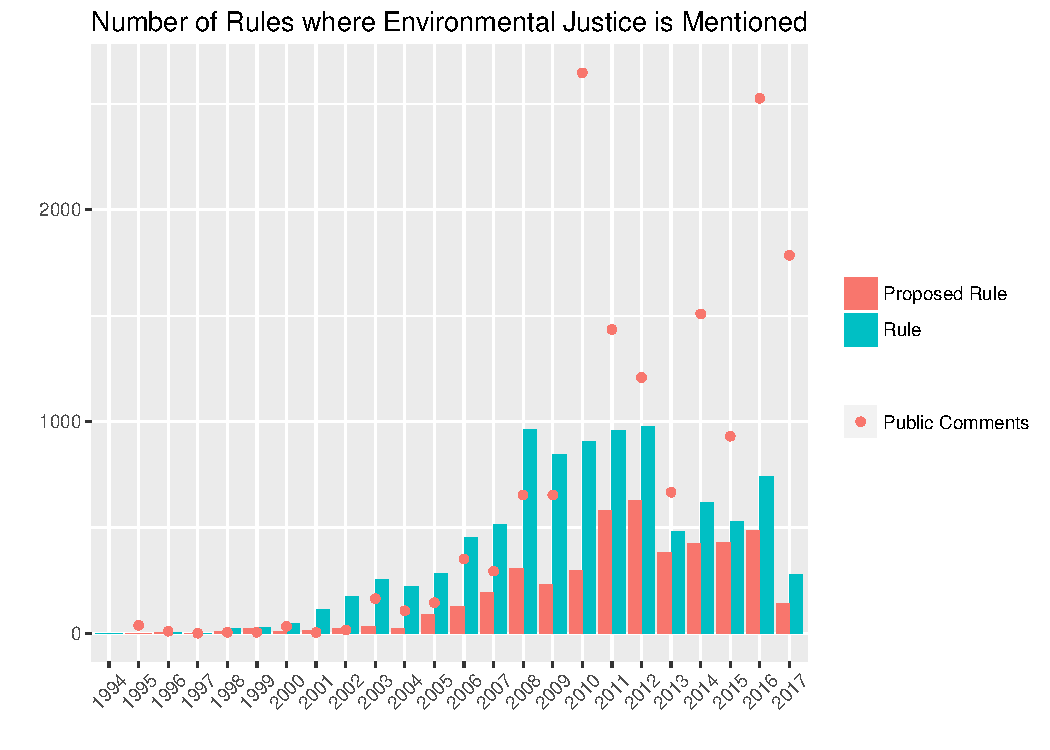
\includegraphics[width = \textwidth/2]{eandj_hist.pdf}
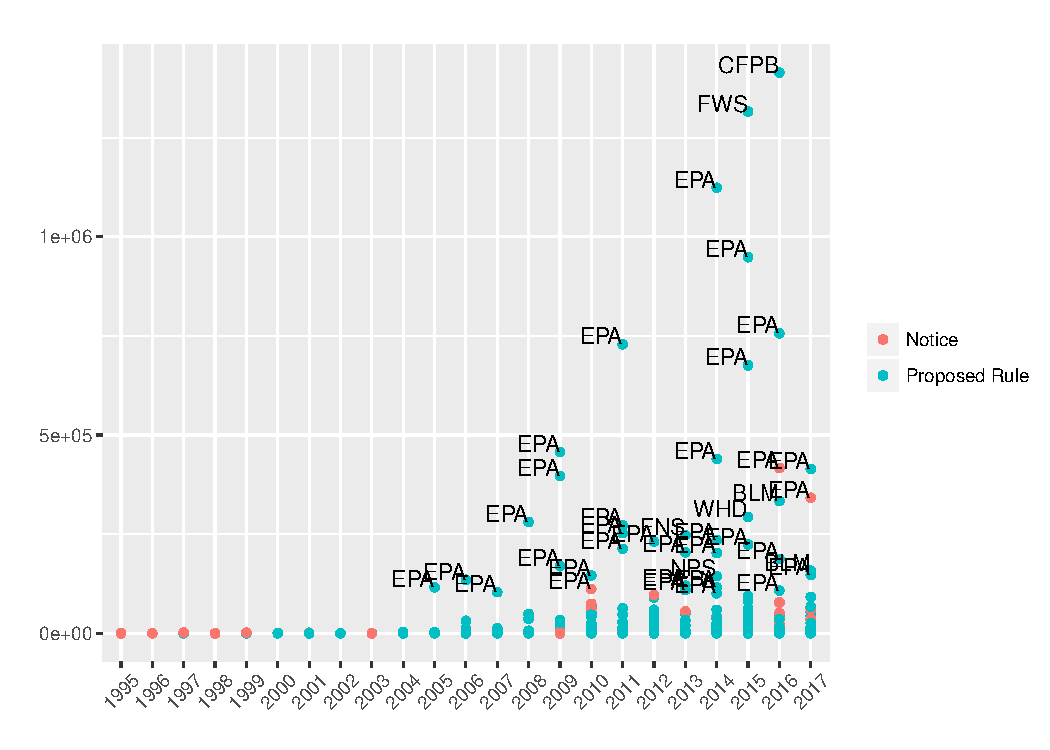
\includegraphics[width =\textwidth/2]{eandj_comments.pdf}
\end{figure}
\end{frame}

\begin{frame}
\frametitle{Win Rate}
\begin{figure}
\caption{Rules With Comments Addressing EJ on a Draft That Did Not}
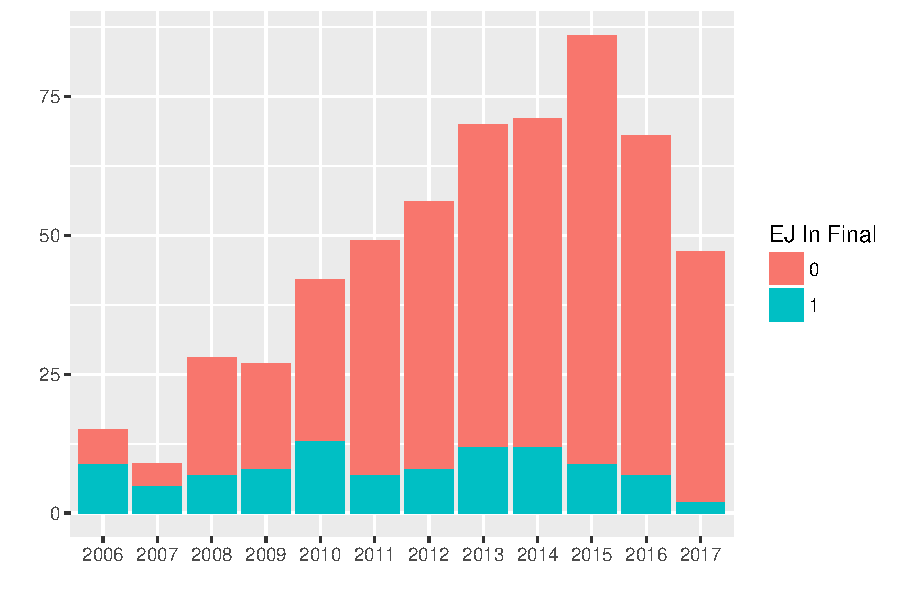
\includegraphics[width = \textwidth/2]{ej_win_rate.pdf}
\end{figure}
\end{frame}

\section{Results}

\begin{frame}
\frametitle{Logit Regression}
\begin{figure}
\caption{Predicted Probability That a Rule Will Address EJ when the Draft Did Not}
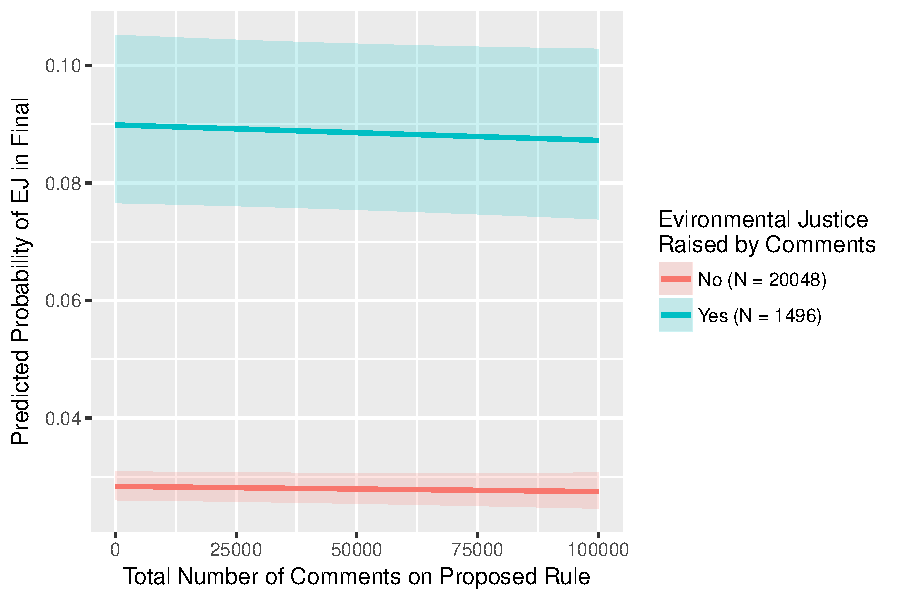
\includegraphics[height = 7cm]{ej_prob_env_nprms.pdf}
\end{figure}
\end{frame}

\begin{frame}
\frametitle{Logit Regression: EPA}
\begin{figure}
\caption{Predicted Probability That a Rule Will Address EJ when the Draft Did Not}
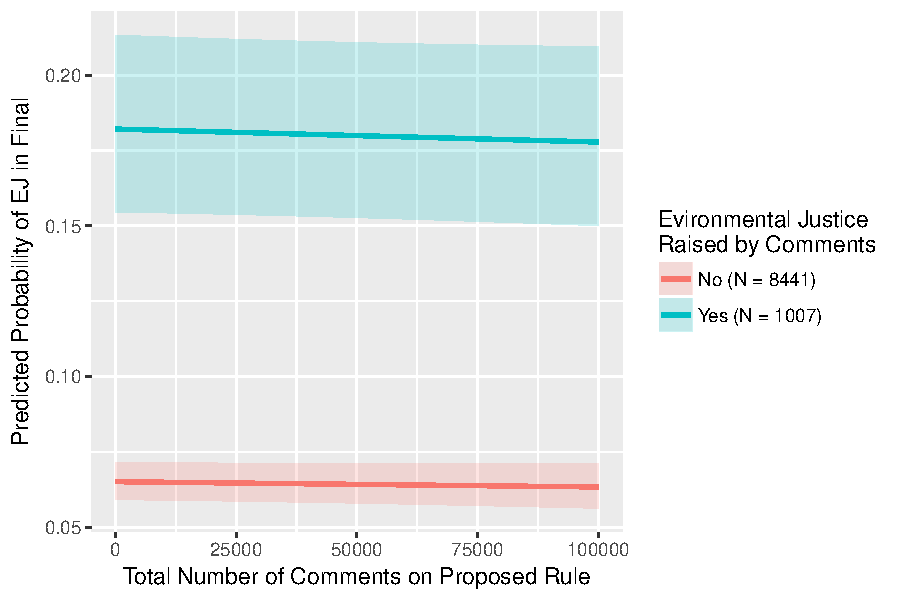
\includegraphics[height = 7cm]{ej_prob_epa_nprms.pdf}
\end{figure}
\end{frame}

\begin{frame}
\frametitle{Probability of Responding to Environmental Justice Claims by Agency}
\begin{figure}
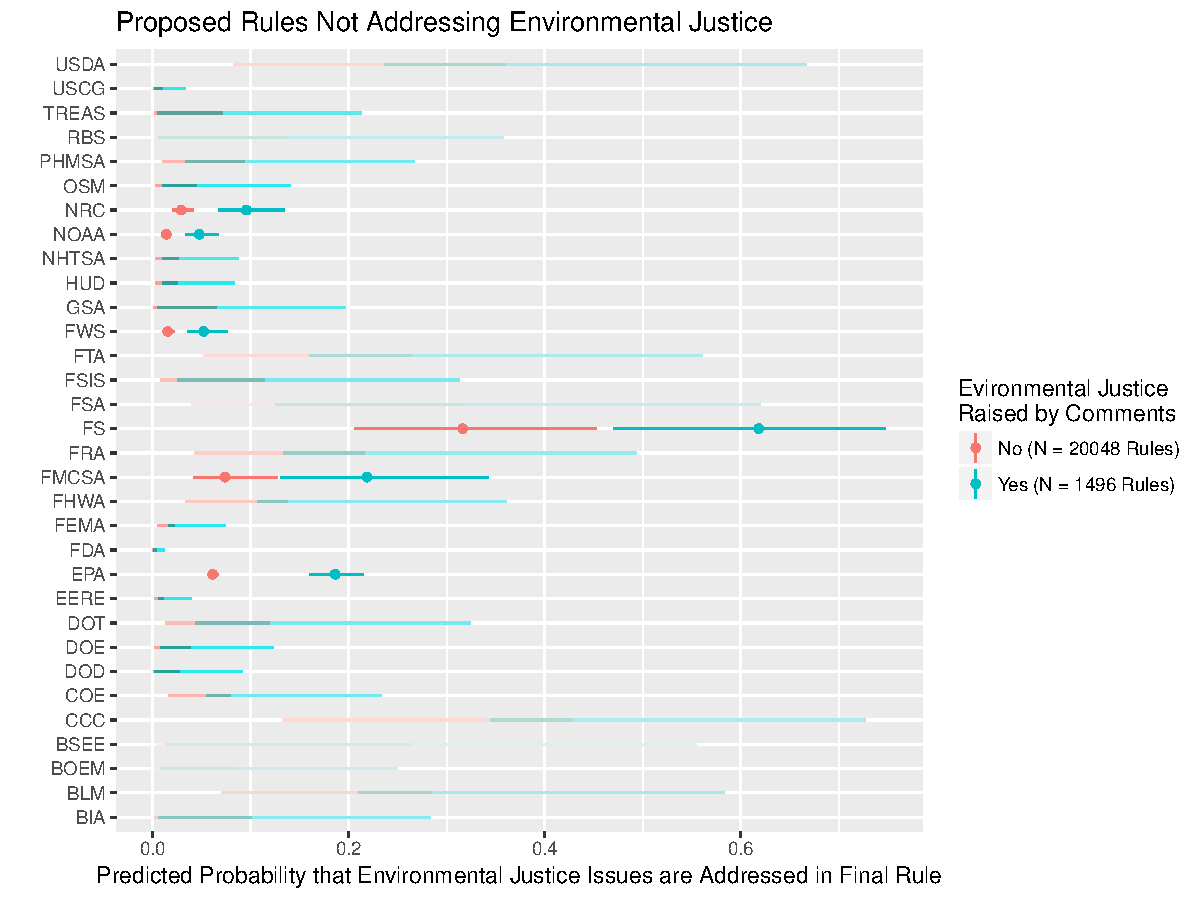
\includegraphics[height = 7.5cm]{ej_prprob_by_agency.pdf}
\end{figure}
\end{frame}

\end{document}











\end{document}